\section{有损优化：缩减 KV Cache}

既然推理是内存受限的，核心优化思路就是\textbf{减少需要传输的内存量}。KV Cache 是推理中最大的内存消耗之一，本节介绍几种在不显著损失精度的前提下缩减 KV Cache 的方法。

\subsection{分组查询注意力（GQA）}

\begin{importantbox}{GQA 的核心思想}
标准多头注意力（MHA）中，每个 Query 头都有对应的 Key 和 Value 头（$K = N$）。GQA 让多个 Query 头\textbf{共享}同一组 Key/Value 头，从而减少 KV Cache 大小。
\begin{itemize}
    \item \textbf{MHA}：$K = N$（每个 Query 头一个 KV 头）
    \item \textbf{MQA}：$K = 1$（所有 Query 头共享一个 KV 头）
    \item \textbf{GQA}：$1 < K < N$（折中方案）
\end{itemize}
\end{importantbox}

\begin{figure}[H]
\centering
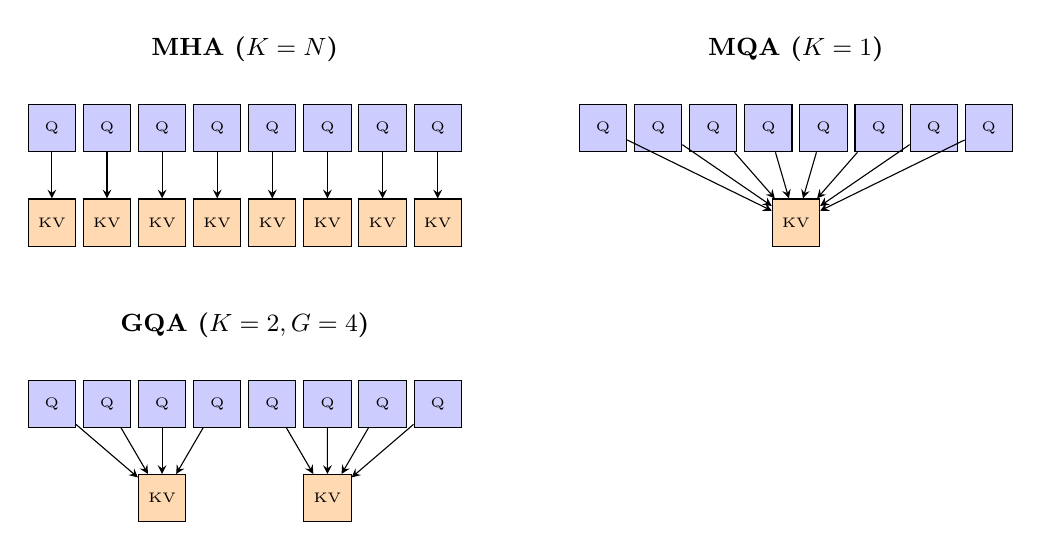
\begin{tikzpicture}[
    qhead/.style={draw, fill=blue!20, minimum width=0.6cm, minimum height=0.6cm, font=\tiny},
    kvhead/.style={draw, fill=orange!30, minimum width=0.6cm, minimum height=0.6cm, font=\tiny},
    arrow/.style={->, thick, >=stealth}
]
% MHA
\node[font=\small\bfseries] at (0, 2.5) {MHA ($K=N$)};
\foreach \i in {0,...,7} {
    \node[qhead] (q1\i) at (\i*0.7-2.45, 1.5) {Q};
    \node[kvhead] (kv1\i) at (\i*0.7-2.45, 0.3) {KV};
    \draw[arrow, thin] (q1\i) -- (kv1\i);
}

% GQA
\node[font=\small\bfseries] at (0, -1) {GQA ($K=2, G=4$)};
\foreach \i in {0,...,7} {
    \node[qhead] (q2\i) at (\i*0.7-2.45, -2) {Q};
}
\node[kvhead] (kv20) at (-1.05, -3.2) {KV};
\node[kvhead] (kv21) at (1.05, -3.2) {KV};
\foreach \i in {0,...,3} { \draw[arrow, thin] (q2\i) -- (kv20); }
\foreach \i in {4,...,7} { \draw[arrow, thin] (q2\i) -- (kv21); }

% MQA
\node[font=\small\bfseries] at (7, 2.5) {MQA ($K=1$)};
\foreach \i in {0,...,7} {
    \node[qhead] (q3\i) at (\i*0.7+4.55, 1.5) {Q};
}
\node[kvhead] (kv30) at (7, 0.3) {KV};
\foreach \i in {0,...,7} { \draw[arrow, thin] (q3\i) -- (kv30); }
\end{tikzpicture}
\caption{MHA、GQA、MQA 的区别：Q 头（蓝）到 KV 头（橙）的映射关系。GQA 是 MHA 和 MQA 之间的折中。}
\end{figure}

GQA 将 KV Cache 缩减为原来的 $K/N$ 倍。以 Llama 2 13B 为例：

\begin{itemize}
    \item 原始配置（$K=40$, $B=64$）：内存约 79 GB，$B=256$ 时超出 H100 容量
    \item 使用 GQA（$K=8$, $B=64$）：内存显著减少，吞吐量大幅提升
    \item 使用 GQA（$K=8$, $B=256$）：现在可以放入 H100 内存，进一步提升吞吐量
\end{itemize}

\begin{table}[H]
\centering
\begin{tabular}{lccccc}
\toprule
\textbf{模型} & \textbf{$N$} & \textbf{$K$} & \textbf{KV Cache/序列} & \textbf{压缩比} & \textbf{$B_\text{max}$（H100）} \\
\midrule
Llama 2 7B (MHA) & 32 & 32 & 1024 MB & 1$\times$ & $\sim$50 \\
Llama 2 70B (GQA) & 64 & 8 & 640 MB & 8$\times$ & $\sim$100 \\
Llama 3 8B (GQA) & 32 & 8 & 256 MB & 4$\times$ & $\sim$200 \\
Llama 3 70B (GQA) & 64 & 8 & 640 MB & 8$\times$ & $\sim$100 \\
Llama 3 405B (GQA) & 128 & 8 & 1280 MB & 16$\times$ & --- \\
\bottomrule
\end{tabular}
\caption{不同 Llama 模型的 KV Cache 大小对比（$S=4096$, bf16）。$B_\text{max}$ 为单 H100 GPU（80GB）上大致可容纳的最大批大小（需同时装下模型参数）。}
\end{table}

\begin{warningbox}{GQA 压缩比 $\neq$ 推理加速比}
GQA 的 $K/N$ 压缩比仅适用于 KV Cache 部分。模型参数大小不变，MLP 层的内存传输量也不变。实际加速比取决于 KV Cache 在总内存传输中的占比——序列越长、KV Cache 占比越大，GQA 的加速效果越明显。
\end{warningbox}

\begin{knowledgebox}{GQA 的精度影响}
实验表明，GQA 在大幅降低推理成本的同时，对模型精度的影响微乎其微。Llama 3 已全面采用 GQA。实际上 Llama 2 的 70B 版本已经使用了 GQA，但较小的模型没有使用。
\end{knowledgebox}

\subsection{多头潜在注意力（MLA）}

MLA（Multi-head Latent Attention）来自 DeepSeek v2，采用与 GQA 不同的策略来缩减 KV Cache。

\begin{importantbox}{MLA 的核心思想}
GQA 通过\textbf{减少 KV 头的数量}来缩减缓存。MLA 则保持头的数量不变，而是将每个 Key/Value 向量\textbf{投影到低维空间}。

具体做法：将每个 token 的 KV 表示从 $N \times H$ 维投影到 $C$ 维（$C \ll N \times H$）。
\end{importantbox}

DeepSeek v2 的配置：
\begin{itemize}
    \item 原始 KV 维度：$N \times H = 16384$
    \item 投影后维度：$C = 512$（压缩比超过 30 倍）
    \item 由于 MLA 与 RoPE 不兼容，需要额外 64 维来编码位置信息，实际为 576 维
\end{itemize}

\begin{knowledgebox}{MLA 的精度表现}
DeepSeek 的实验表明：
\begin{enumerate}
    \item MHA 优于 GQA（精度更高，但开销也更大）
    \item MLA 比 MHA 精度略好，同时推理开销远低于 MHA
\end{enumerate}
MLA 在精度-效率的帕累托前沿上优于 GQA 和 MHA。
\end{knowledgebox}

\begin{warningbox}{MLA 与 RoPE 的兼容性问题}
MLA 将 KV 向量投影到低维空间后再存储。但 RoPE 位置编码作用于原始 Key 向量——如果先投影再加 RoPE，则无法从低维表示恢复带位置信息的 Key。DeepSeek v2 的解决方案是为每个 token 额外存储 64 维的``解耦 RoPE Key''，使实际缓存维度从 512 增加到 576。这一工程细节在实现 MLA 时容易被忽略。
\end{warningbox}

\subsection{跨层注意力（CLA）}

\begin{importantbox}{CLA 的核心思想}
GQA 在\textbf{头}的维度上共享 KV 向量，CLA 则在\textbf{层}的维度上共享——让多个相邻层共享同一组 KV Cache。
\end{importantbox}

实验表明，CLA 能够在精度与 KV Cache 大小之间改善帕累托前沿。CLA 可以与 GQA 叠加使用，进一步缩减缓存。

\subsection{局部注意力}

\begin{importantbox}{局部注意力（滑动窗口注意力）}
核心思想：每个 token 只关注局部上下文（最近的 $w$ 个 token），而非全部历史。
\begin{itemize}
    \item 有效上下文随层数线性增长
    \item KV Cache 大小\textbf{不再依赖序列长度}——变为常数
\end{itemize}
\end{importantbox}

\begin{warningbox}{局部注意力的精度损失}
纯局部注意力会损失对远距离依赖的建模能力。解决方案：\textbf{混合架构}——交替使用局部注意力层和全局注意力层。例如 character.ai 每 6 层使用 1 层全局注意力（结合 CLA），在大幅降低推理成本的同时保持了良好的精度。Mistral 7B 也采用了滑动窗口注意力。
\end{warningbox}

\subsection{本章小结}

缩减 KV Cache 的核心策略包括：
\begin{enumerate}
    \item \textbf{减少 KV 头数量}：GQA（头间共享）
    \item \textbf{降低 KV 维度}：MLA（低秩投影）
    \item \textbf{跨层共享}：CLA（层间共享）
    \item \textbf{限制注意力范围}：局部注意力（固定窗口）
\end{enumerate}
这些方法可以组合使用，且实验表明对精度的影响可控。所有方法都直接转化为更低的延迟和更高的吞吐量，因为推理是内存受限的。

\begin{table}[H]
\centering
\begin{tabular}{lcccc}
\toprule
\textbf{方法} & \textbf{压缩维度} & \textbf{典型压缩比} & \textbf{精度影响} & \textbf{代表模型} \\
\midrule
GQA & 头间共享 & 4--16$\times$ & 极小 & Llama 2/3 \\
MQA & 头间共享（极端） & $N\times$ & 小--中等 & PaLM, Gemini \\
MLA & 低秩投影 & $>$30$\times$ & 极小（甚至提升） & DeepSeek v2/v3 \\
CLA & 层间共享 & 2--4$\times$ & 小 & character.ai \\
局部注意力 & 限制序列范围 & $\propto w/S$ & 中等（需混合） & Mistral 7B \\
\bottomrule
\end{tabular}
\caption{KV Cache 优化方法量化对比。压缩比为相对于标准 MHA 的缩减倍数。这些方法可以叠加使用。}
\end{table}

%% ========== Section 4: Transformer 的替代架构 ==========

